\documentclass[tikz]{standalone}
\begin{document}
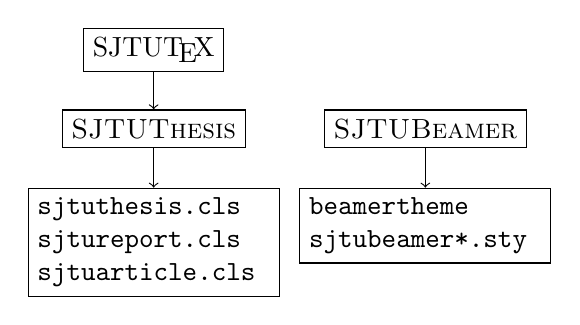
\begin{tikzpicture}
  \node[draw] (v1) at (-0.5,1.5) {SJTU\TeX{}};
  \node[draw,font=\scshape] (v2) at (-0.5,0.5) {SJTUThesis};
  \node[draw,font=\scshape] (v4) at (2.95,0.5) {SJTUBeamer};
  \draw[->]  (v1) edge (v2);
  \node[draw,font=\ttfamily,anchor=north] (v3) at (-0.5,-0.25) {\parbox{8em}{sjtuthesis.cls\\sjtureport.cls\\sjtuarticle.cls}};
  \draw[->]  (v2) edge (v3);
  \node[draw,font=\ttfamily,anchor=north] (v5) at (2.95,-0.25) {\parbox{8em}{beamertheme\\sjtubeamer*.sty}};
  \draw[->]  (v4) edge (v5);
\end{tikzpicture}
\end{document}
